\scanpage{57}
\margin{\figure{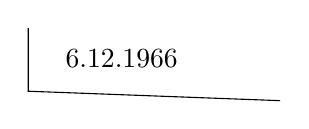
\begin{tikzpicture}
\draw (0,0.8)--(0,0)--(3.2,-0.12);
\node[anchor=west] at (0.35,0.42) {6.12.1966};
\end{tikzpicture}}}
\uline{Laïus}

\margin{\diagram{\begin{tikzcd}[ampersand replacement=\&]
X \arrow[d,"f"']\\
S
\end{tikzcd}}}
Soit $\mathcal{F}$ un Module quasi-cohérent stratifié sur $X/S$.
On a vu qu'il définit un module de $X_{\mathrm{strat}}$, et par là un faisceau cosimplicial
\inserted{\figure{\begin{tikzpicture}
\node[draw,ellipse,inner sep=4pt] {$\mathcal{F}^*=C(\mathcal{F})$};
\end{tikzpicture}}}
sur $X_{\mathrm{zar}}$, par
\[
C^n(\mathcal{F})=\mathcal{F}^{(n)}
=\varprojlim_i\mathcal{F}_{\Delta^n_{X/S}(i)}
\]
[pour n'importe laquelle des $n+1$ projections $\Delta^n_{X/S}(i)\to X$ on prend pour définir l'image inverse, il y a des isoms canoniques entre eux, précisément à cause de la stratification de $\mathcal{F}$].
On a
\[
\boxed{H^*(X_{\mathrm{str}},\mathcal{F})
\simeq\mathbb{H}^*(X_{\mathrm{zar}},C^*(\mathcal{F}))}
\]
On voit donc deux théories cohomologiques;
\deleted{\unsure{pour} \inserted{\unsure{chacune}} \unsure{aucune|encore} ne semble \illegible{1} à première vue, \unsure{purement} \illegible{3} \unsure{pour construire l'autre}.}

a) Pour un $\mathcal{F}$ quasi-cohérent sur $X$, on forme les $H^i(X_{\mathrm{zar}},\mathcal{F})$.

b) Si $\mathcal{F}$ est \uline{stratifié}, on forme les $H^i(X_{\mathrm{strat}},\mathcal{F})$, qui s'explicitent par la formule plus haut.

À première vue, le lien entre ces deux théories cohomologiques semble donné exclusivement par

\margin{56}
